\ifthenelse{\equal{\Langue}{FR}}{
\chapter{Alimentation Flyback}
}{
\chapter{Flyback Power Supply}
}

\ifthenelse{\equal{\Langue}{FR}}{
La maquette d'étude comprend, outre le circuit de commande du transistor, le montage suivant:
}{
The hardware setup includes, in addition to the transistor control circuit, the following assembly:
}

\begin{figure}[h]
\centering
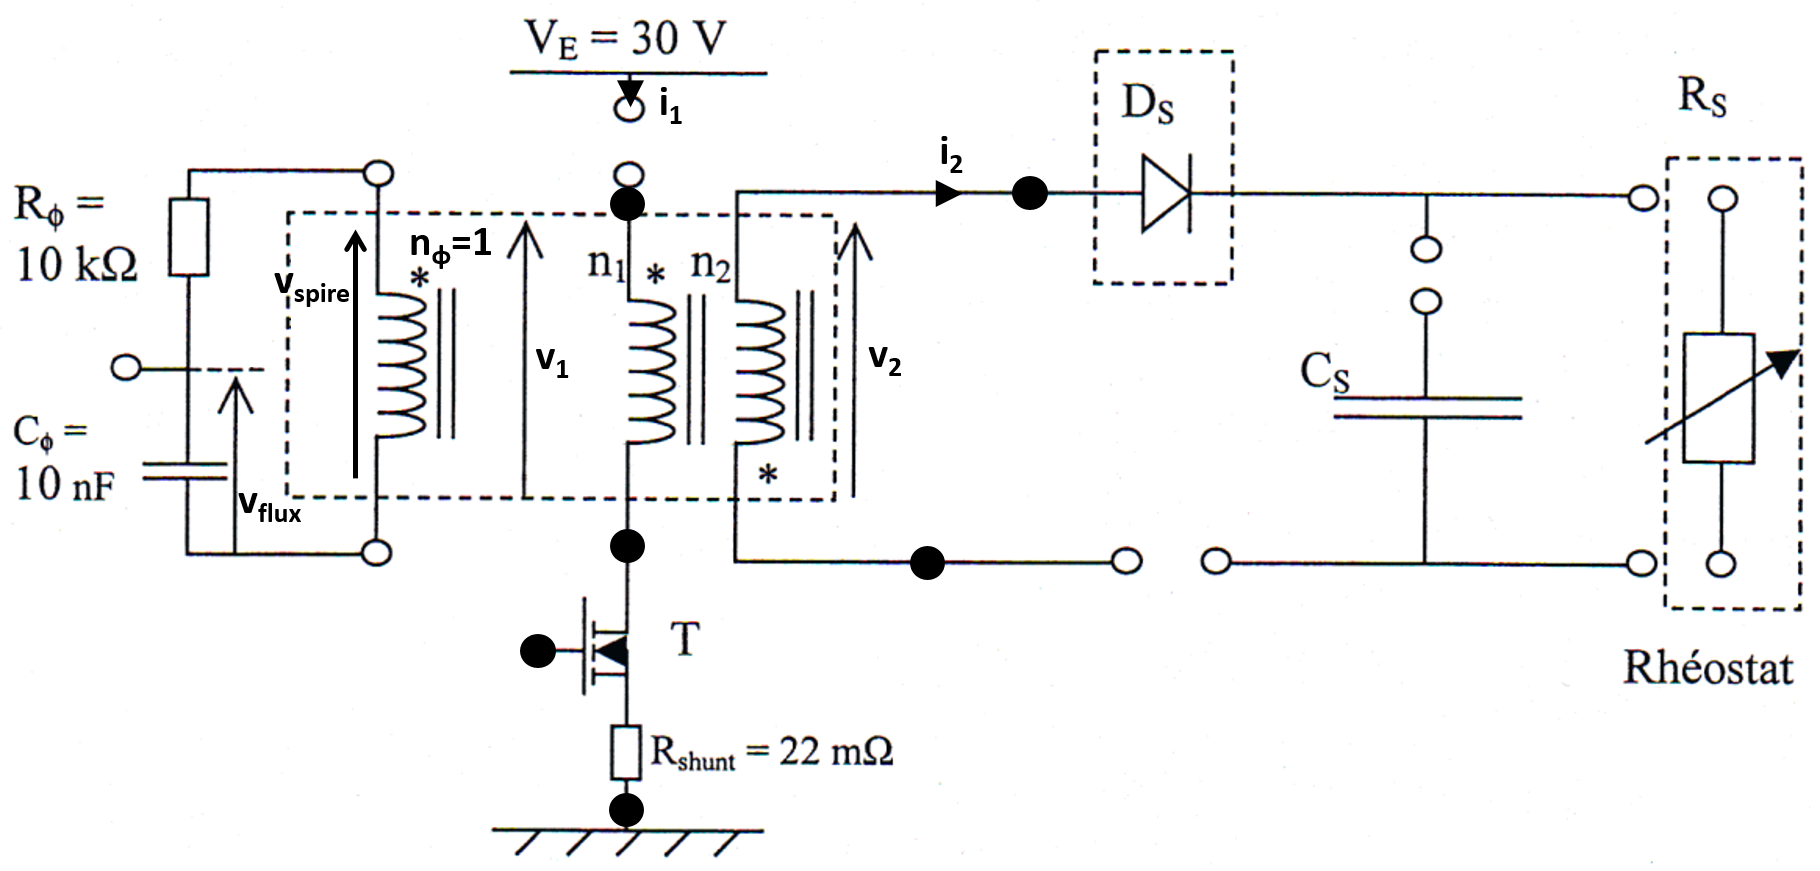
\includegraphics[width=\linewidth]{TP_Flyback/fig/Schema_Flyback.png}
%\caption{Simplified internal control}
\end{figure}

\ifthenelse{\equal{\Langue}{FR}}{
Des pointes de tests $\bullet$ permettent de visualiser les différents signaux, notamment le signal de commande du transistor MOSFET\@.

Les 3 enroulements sont sur le même noyau magnétique ETD29/16/10 réalisé avec une ferrite de type N27 dont la document est en annexe. Ce noyau peut être muni d'un entrefer réglé par des cales amagnétiques. Dans ce cas, la relation entre l'épaisseur $s$ de l'entrefer et la valeur $A_L$ de l'inductance spécifique est donnée par la relation suivante où $K_1$ et $K_2$ sont deux constantes données dans la documentation:
}{

Test points $\bullet$ allow visualization of the different signals, including the control signal of the MOSFET transistor.

The 3 windings are on the same ETD29/16/10 magnetic core made of N27 type ferrite, which documentation is in the appendix. This core can be equipped with an air gap adjusted by non-magnetic shims. In this case, the relationship between the thickness $s$ of the air gap and the value $A_L$ of the specific inductance is given by the following relation where $K_1$ and $K_2$ are two constants given in the documentation:
}
\[s={\left(\dfrac{A_L}{K_1}\right)}^{\dfrac{1}{K_2}}\]

\ifthenelse{\equal{\Langue}{FR}}{
Les liaisons manquantes devront être réalisées par des ``cavaliers'' permettant de visualiser les courants par l'utilisation de sondes appropriées. Le rhéostat de charge peut être de 250 $\Omega$ ou 330 $\Omega$ indifféremment et on veillera à \underline{\textbf{ne pas brancher la tension $V_E$ sans la présence}} \underline{\textbf{de cette charge}}.

On notera la présence d'un circuit de mesure du flux réalisé par une spire unique reliée à un circuit R-C intégrateur. La tension $v_{flux}$ permet donc de visualiser l'ondulation du flux dans le circuit magnétique.
}{
The missing connections must be made by ``jumpers'' allowing the currents to be visualized by the use of appropriate probes. The load rheostat can be either 250 $\Omega$ or 330 $\Omega$ and care should be taken \underline{\textbf{not to connect the voltage $V_E$ without the presence of this load}}.

It should be noted that there is a flux measurement circuit made up of a single turn connected to an R-C integrator circuit. The voltage $v_{flux}$ therefore allows the ripple of the flux in the magnetic circuit to be visualized.
}
\newpage
\ifthenelse{\equal{\Langue}{FR}}{
Le dispositif de commande du transistor est représenté sur la figure ci dessous:
}{
The transistor control device is shown in the figure below:
}

\begin{figure}[h]
\centering
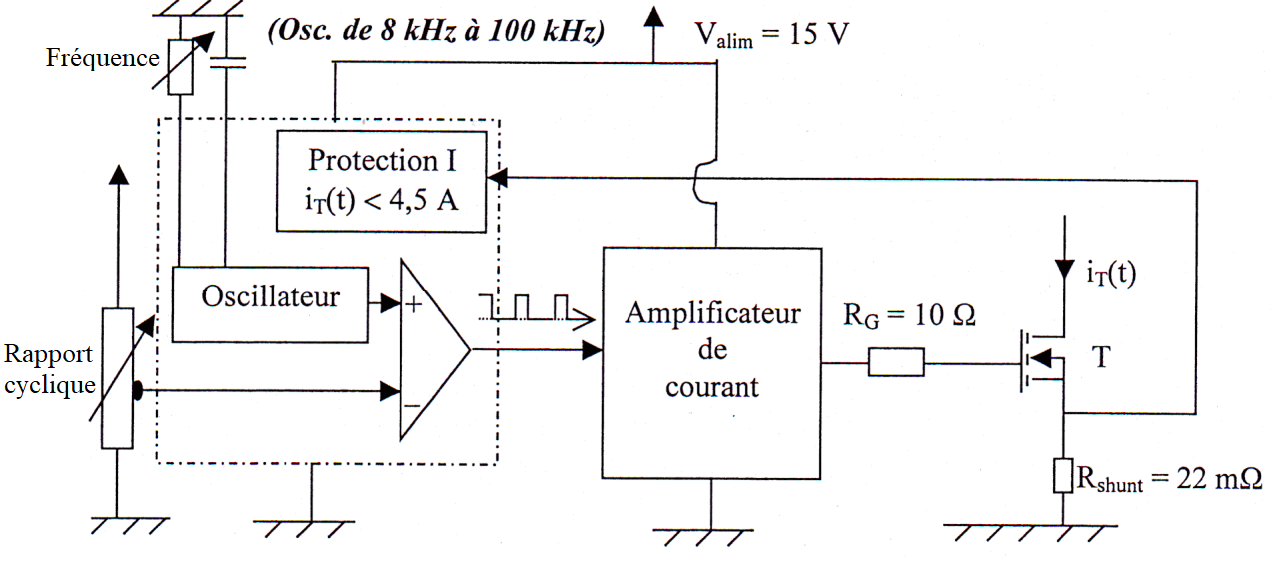
\includegraphics[width=\linewidth]{TP_Flyback/fig/Control_Flyback.png}
%\caption{Simplified internal control}
\end{figure}

\ifthenelse{\equal{\Langue}{FR}}{
Un potentiomètre permet de régler la fréquence (ne pas descendre en dessous de 15 kHz), un second permet de régler le rapport cyclique. Ce dernier est muni d'une limitation de courant active réglée à 4,5A et réalisée par la mesure de tension sur un shunt de 22 m$\Omega$. L'alimentation de cette commande est réalisée par une source de tension indépendante de valeur $V_{alim} = 15 V$.
}{
A potentiometer allows the frequency to be adjusted (do not go below 15 kHz), a second allows the duty cycle to be adjusted. The latter is equipped with an active current limit set to 4.5A and implemented by measuring the voltage across a 22 m$\Omega$ shunt. The power supply for this control is provided by an independent voltage source of value $V_{alim} = 15 V$.
}
\newpage
\ifthenelse{\equal{\Langue}{FR}}{
\section{Préparation}
}{
\section{Preparation}
}

\ifthenelse{\equal{\Langue}{FR}}{
On suppose que le transistor est commandé par un signal PWM de rapport cyclique $\alpha=0.25$. On suppose également que le convertisseur fonctionne en \textbf{régime de démagnétisation totale} pour le transformateur. La tension d'entrée $V_E$ est supposée constante. On étudiera pour la préparation uniquement le \underline{régime permanent}.
}{
We assume that the transistor is controlled by a PWM signal with a duty cycle of $\alpha=0.25$. We also assume that the converter operates in \textbf{total demagnetization mode} for the transformer. The input voltage $V_E$ is assumed to be constant. For preparation, we will only study the \underline{steady state}.
}

\begin{enumerate}
\ifthenelse{\equal{\Langue}{FR}}{
\item Compléter les chronogrammes ci-dessous en traçant: 
}{
\item Complete the chronograms below by drawing:
}
\begin{itemize}
\ifthenelse{\equal{\Langue}{FR}}{
\item le flux $\varphi$ dans le transformateur
\item le courant $i_1$ délivré par l'alimentation
\item le courant $i_2$ dans la diode
\item la tension $v_2$ en sortie du transformateur
}{
\item the flux $\varphi$ in the transformer
\item the current $i_1$ delivered by the power supply
\item the current $i_2$ in the diode
\item the voltage $v_2$ at the output of the transformer
}
\end{itemize}


\begin{figure}[h]
\centering

\includegraphics[width=0.7\linewidth]{TP_Flyback/fig/prepa.png}
%\caption{Simplified internal control}
\end{figure}

\ifthenelse{\equal{\Langue}{FR}}{
\item On suppose que la constante de temps du filtre $R_\phi-C_\phi$ est grande devant la période de découpage du hacheur. Montrer que $v_{flux}$ permet de visualiser l'ondulation de flux dans la transformateur. Déterminer l'ondulation de flux $\Delta \varphi$ en fonction de $\alpha$, $T$ et la valeur de $v_{spire}$ sur l'intervalle $0<t<\alpha T$.
}{
\item We assume that the time constant of the filter $R_\phi-C_\phi$ is large compared to the switching period of the chopper. Show that $v_{flux}$ allows visualizing the flux ripple in the transformer. Determine the flux ripple $\Delta \varphi$ as a function of $\alpha$, $T$ and the value of $v_{spire}$ over the interval $0<t<\alpha T$.
}
\end{enumerate}


%%%%%%%%%%%%%%%%%

\newpage
\ifthenelse{\equal{\Langue}{FR}}{
Durant tout le TP, les précautions suivantes devront être prises:
}{
For the entire lab session, the following precautions must be taken:
}

\begin{itemize}
\ifthenelse{\equal{\Langue}{FR}}{
\item utiliser deux sources indépendantes pour réaliser $V_{alim}$ et l'alimentation ``de puissance'' $V_E$: \textbf{on
règlera soigneusement la limitation de courant de celle-ci à 2 A}
\item laisser la tension $V_{alim}$ présente durant toute la séance mais baisser la tension $V_E$ à chaque
modification de branchement
\item ne pas abaisser la fréquence de découpage en dessous de 15 kHz
\item lorsque plusieurs mesures de tensions sont réalisées en même temps avec une sonde de tension, \textbf{attention à ne pas réaliser de court-circuit}. En effet, les sondes de tensions ne sont pas isolées entre elles, les références de potentiel des sondes sont donc liées via l'oscilloscope
}{
\item use two independent sources to realize $V_{alim}$ and the ``power'' supply $V_E$: \textbf{the current limit will be carefully set to 2 A}
\item keep the voltage $V_{alim}$ present during the entire session but reduce the voltage $V_E$ at each
connection modification
\item do not lower the switching frequency below 15 kHz
}
\end{itemize}

\ifthenelse{\equal{\Langue}{FR}}{
\section{Étude magnétique, formes d'onde}
}{
\section{Magnetic Study, Waveforms}
}

\ifthenelse{\equal{\Langue}{FR}}{
On effectuera les mesures suivantes avec le rhéostat de charge à sa valeur maximale (charge réduite) et en veillant à travailler en régime de démagnétisation totale, pour un rapport cyclique voisin de sa valeur maximale.
}{
Perform the following measurements with the load rheostat at its maximum value (reduced load) and by ensuring to work in the total demagnetization mode, for a duty cycle close to its maximum value.
}

\begin{enumerate}
\ifthenelse{\equal{\Langue}{FR}}{
\item Régler la fréquence de découpage à 50 kHz et le rapport cyclique à sa valeur maximale (que l'on notera). Observer la tension aux bornes de la spire de mesure du flux $v_{spire}$ ainsi que la tension $v_{flux}$. En déduire l'excursion crête à crête $\Delta B$ de l'induction magnétique dans le circuit en s'aidant de la documentation ($\Delta B = B_{\max} - B_{\min}$).
\item Par comparaison des tensions $v_{spire}$ et $v_1$, puis $v_2$, déterminer les nombres de spires $n_1$ et $n_2$.
\item Observer simultanément les courants $i_1$ et $i_2$ et les comparer à l'évolution du flux.
\item En déduire la valeur de l'inductance magnétisante au primaire, notée $L_1$.
\item A partir des mesures de $n_1$ et $L_1$ et en utilisant la documentation, déterminer la valeur de l'inductance spécifique $A_L$ puis l'épaisseur de l'entrefer. Quel est le rôle de cet entrefer?
}{
\item Set the switching frequency to 50 kHz and the duty cycle to its maximum value (which will be noted). Observe the voltage across the flux measurement turn $v_{spire}$ as well as the voltage $v_{flux}$. Deduce the peak-to-peak excursion $\Delta B$ of the magnetic induction in the circuit using the documentation ($\Delta B = B_{\max} - B_{\min}$).
\item By comparing the voltages $v_{spire}$ and $v_1$, then $v_2$, determine the number of turns $n_1$ and $n_2$.
\item Observe simultaneously the currents $i_1$ and $i_2$ and compare them to the evolution of the flux.
\item Deduce the value of the magnetizing inductance at the primary, denoted $L_1$.
\item From the measurements of $n_1$ and $L_1$ and using the documentation, determine the value of the specific inductance $A_L$ and then the thickness of the air gap. What is the role of this air gap?
}
\end{enumerate}

\newpage
\ifthenelse{\equal{\Langue}{FR}}{
\section{Courbes statiques}
}{
\section{Static Curves}
}

\ifthenelse{\equal{\Langue}{FR}}{
Le but de ces mesures est de relever le réseau des caractéristiques statiques en sortie de l'alimentation. La fréquence de découpage est dans un premier temps maintenue constante égale à 50 kHz.
}{
The purpose of these measurements is to record the network of static characteristics at the output of the power supply. The switching frequency is initially kept constant at 50 kHz.
}


\begin{enumerate}
\ifthenelse{\equal{\Langue}{FR}}{
\item Pour plusieurs valeurs du rapport cyclique (par exemple $\alpha_{\max}$, 0.3, 0.2 et 0.1), modifier la résistance du rhéostat de charge pour faire varier le courant moyen débité entre sa valeur minimale (obtenue avec le rhéostat au maximum) et une valeur maximale de 2 A. Relever alors les valeurs moyennes du courant débité par l'alimentation de puissance $V_E$, $I_E$, du courant de sortie, $I_S$, et de la tension de sortie, $V_S$. Noter soigneusement le point de fonctionnement correspondant au changement de régime de l'alimentation vis à vis de la démagnétisation.
\item En déduire le tracé des caractéristiques $V_S(I_S)$ et $P_S(I_S)$ (puissance de sortie) paramétrées par $\alpha$. Tracer également les caractéristiques de transfert en puissance $P_S(P_E)$ et en déduire le rendement. Faire apparaître les zones de fonctionnement en démagnétisation partielle et en démagnétisation totale.
%\item Afin de maintenir l'alimentation en régime critique, il est possible de modifier la fréquence de découpage. Ceci est en général réalisé au moyen d'une commande auto-oscillante mais on peut simuler ce fonctionnement de la façon suivante : on réglera la fréquence de découpage pour maintenir la valeur moyenne de la tension de sortie constante alors que le rapport cyclique reste constant, réglé à $\alpha_{max}$, ceci pour différentes valeurs du rhéostat de charge. Pour réaliser facilement ces mesures, on procédera ``à l'envers'' en réglant d'abord une valeur de fréquence de découpage puis en modifiant la valeur du rhéostat pour obtenir la tension de sortie souhaitée, par exemple $V_S = 40 V$. Relever alors le point de fonctionnement, i.e. la valeur moyenne du courant de sortie $I_S$ et la fréquence de découpage.
%\item Observer les formes d'onde de la tension $V_{CE}$ aux bornes du transistor et du courant $i_1$ le traversant. En déduire les contraintes sur la transistor.
}{
\item For several values of the duty cycle (for example $\alpha_{\max}$, 0.3, 0.2 and 0.1), modify the resistance of the load rheostat to vary the average current delivered between its minimum value (obtained with the rheostat at maximum) and a maximum value of 2 A. Then record the average values of the current delivered by the power supply $V_E$, $I_E$, the output current, $I_S$, and the output voltage, $V_S$. Carefully note the operating point corresponding to the change in regime of the power supply with respect to demagnetization.
\item Deduce the plot of the characteristics $V_S(I_S)$ and $P_S(I_S)$ (output power) parameterized by $\alpha$. Also plot the power transfer characteristics $P_S(P_E)$ and deduce the efficiency. Show the operating zones in partial demagnetization and total demagnetization.
}
\end{enumerate}

\ifthenelse{\equal{\Langue}{FR}}{
\section{Mesures complémentaires}
}{
\section{Additional Measurements}
}

\ifthenelse{\equal{\Langue}{FR}}{
Laisser le rhéostat de charge à sa valeur maximale et la fréquence de découpage à 50 kHz.
}{
Keep the load rheostat at its maximum value and the switching frequency at 50 kHz.
}

\begin{enumerate}
\ifthenelse{\equal{\Langue}{FR}}{
\item Observer simultanément le courant $i_1$ et la tension aux bornes du transistor $v_T$. En déduire les contraintes subies par ce transistor.% et évaluer ses pertes en commutation et en conduction.
\item Observer simultanément le courant dans le condensateur de filtrage $I_{CS}$ et la tension de sortie $v_S$. En déduire la valeur du condensateur de filtrage $C_S$.
}{
\item Observe simultaneously the current $i_1$ and the voltage across the transistor $v_T$. Deduce the stresses experienced by this transistor.% and evaluate its switching and conduction losses.
\item Observe simultaneously the current in the filter capacitor $I_{CS}$ and the output voltage $v_S$. Deduce the value of the filter capacitor $C_S$.
}

\end{enumerate}
